\documentclass[a4paper,12pt]{report}
    \title{Service Registry}
\author{Theodor Bogdan Vr\^ancean}
\date {Iunie 2018}

\usepackage[romanian]{babel}

\usepackage{graphicx}
\graphicspath{{"./Images/"}}

\usepackage[
    backend=biber,
    style=verbose,
	sorting=ynt,
	maxbibnames=99,
	maxcitenames=6
]{biblatex}
\addbibresource{References.bib}

\begin{document}
\maketitle
\tableofcontents
\chapter{Introducere}
\section{Arhitectura de microservicii}

Arhitectura de microservicii este o abrodare relativ nou\u a \^ in dezvoltarea de software.
Microserviciile reprezint\u a aplica\c tii mici \c si autonome care lucreaz\u a \^ impreun\u a
\footcite{buildingMicroservices1}. Ele sunt considerate mici relativ la un sistem monolitic care ar
oferi toate func\c tionalit\u a\c tiile de care aplica\c tia are nevoie.Cu toate acestea un mictoserviciu poate oferi orice
fel de func\c tionalit\u a\c ti,incep\^and cu ceva simplu precum desc\u arcarea de fi\c siere, p\^an\u a la
complexe precum analizarea imaginilor.
Aceast\u a aboradare arhitecturala a venit ca o alternativ\u a la arhitectura monolitic\u a, \^in care exist\u a
un singur server care satisface toate necesit\u a\c tile unei aplica\c tii.Limit\u arile acestei abord\u ari ies la iveal\u a
odat\u a cu cre\c sterea aplica\c tiei.
Pentru a \^intelege de ce arhitectura  de microservicii \^incepe sa \^inlocuiasc\u a arhitectura monolitic\u a
trebuie sa cunoa\c stem urm\u atoarele beneficii:
\begin{itemize}
	\item Din cauza dimensiunii \c si complexit\u a\c tii unui proiect monolitic,
	      acesta este dificil de in\c teles \c ,motiv pentru care schimb\u arile sunt mai dificil de facut \c si exist\u a
	      un risc mai mare ca acestea s\u a produc\u a efecte nedorite.Aceste probleme pot fi atenuate printr-un
	      cod de calitate dar acest lucru se \^ inatmpla de prea pu\c tine ori. Schimb\u arile aduse unui microserviciu nu afecteaz\u a alte
	      module \c si datorit\u a dimensiunii reduse a acestora, ele sunt \c si mai u\c sor de \^inteles pentru programtori, astfel
	      scade probabilitatea erorilor.Se poate spune ca microserviciile duc un pas mai departe principiul singurei responsabilit\u a\c ti,
	      definit de Robert C. Martin.
	\item Pentru dezvoltarea unei aplica\c tii monolitice trebuie sa alegem tehnologii standardizate care s\u a poata
	      realiza toate cerin\c tele aplica\c tiei. Pe de alta parte,daca avem mai multe microservicii care colaboreaz\u a nu exist\u a
	      aceast\u a limitare,ceea ne permite s\u a alegem unealta cea mai portivit\u a pentru fiecare serviciu.
	      S\u a lu\u am spre exemplu un site al unei pizzerii care folose\c ste microservicii (Fig 1).
	      Partea de front-end doar apeleaz\u a serviciile c\^and are nevoie.Putem avea un server scris
	      in C\# care folose\c ste un sistem de gestiune a bazei de date Microsoft Sql Server,
	      unul scris \^in php cu MySql \c si unul scris in Node.js cu mongoDb \ref{fig:PizzaMicroservicii}.Deoarce toate comunic\u a prin
	      protocolul http ,acestea pot lucra \^impreun\u a,fiecare av\^and responsabilitatea sa.
	      \begin{figure}[!htb]
		      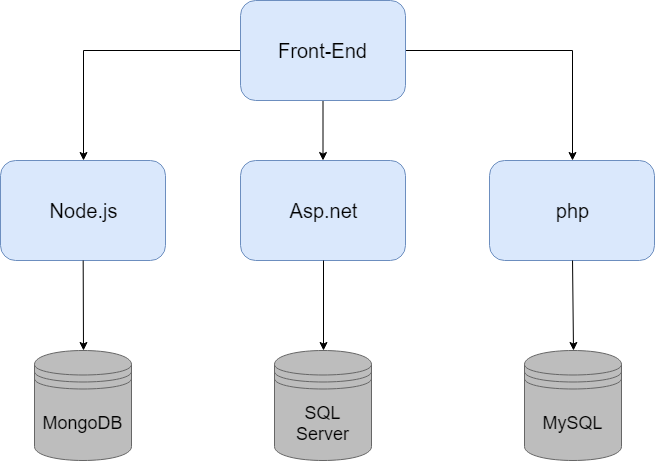
\includegraphics[width=\textwidth,keepaspectratio]{PizzaMicroservicii}
		      \caption{Arhitectur\u a cu microservicii pentru un site de pizzerie}
		      \label{fig:PizzaMicroservicii}
	      \end{figure}
	\item O aplica\c tie a c\u arei componente sunt distribuite este mai rezistent\u a, \^in sensul c\u a dac\u a un
	      serviciu este compromis, func\c tionalita\c tile care nu depind de acel serviciu vor continua s\u a func\c tioneze.
	      \^In cazul unei aplica\c tii clasice, tot sistemul va fi compromis din cauza unei singure componente.
	\item Cu un serviciu mare,monolitic, trebuie sa scal\u am totul \^imreun\u a.O parte mic\u a
	      a \^intregului nostru sistem, este constr\^ans\u a \^in performan\c t\u a, dar dac\u a
	      acest comportament este blocat \^intr-o aplica\c tie monolitic\u a gigant\u a, trebuie sa scal\u am totul \^impreun\u a
	      ca o bucat\u a \footcite{buildingMicroservices5}.Acest lucru se face deobicei folosind mai multe servere
	      \c si un server de tip load balancer care s\u a distribuie cererile c\u atre unul din acele servere pentru
	      a reduce munca depus\u a de un singur server o depune, astfel evit\^and supra\^incarcarea si cresc\^and performan\c ta.
	      \^In cazul arhitecturii cu microservicii, ajunge s\u a scalam doar acele servicii care au probleme de performan\c ta.
	\item Microserviciile ofer\u a \c si reutilizabiliate, ele pot fi utilizate de multiple aplica\c tii.
		  Daca dou\u a aplica\c tii au func\c tionalita\c ti similare, acestea nu trebuie implementate de dou\u a ori, aceast\u a func\c tionalitate
		  poate fi oferit\u a de un serviciu comun , folosit de ambele aplica\c tii.Uneori acest lucru este chiar necesar, dac\u a un produc\u ator de software
		  are mai multe aplica\c tii ce necesit\u a autentificare, este mult mai comod pentru utilizator s\u a aib\u a un singur cont cu care s\u a se autentifice in fiecare aplica\c tie 
		  \c si acest lucru este avantajos si pentru produc\u ator.
		  Microserviciile pot fi f\u acute \c si publice, pe baza unei chei de autentificare,pe care le pot folosi pentru aplica\c tiile lor,persoane in afara companiei produc\u atoare.
		  \^In prezent exist\u a multe servicii de meteorologie, gratuite sau contra cost, pe care le putem folosi \^in aplica\c tiile noastre.
\end{itemize}

Bine\^in\c teles arhitectura cu microservicii nu este o solu\c tie miraculoas\u a la toate problemele,
adat\u a cu aceste beneficii, ea vine \c si cu dezavantajele.Fiind un sistem distribuit toate
problemele acestor sisteme afecteaz\u a si microservicii.
O problem\u a este men\c tinerea leg\u aturii \^intre componentele aplica\c tiei.Un serviciu \^isi poate schimba 
adresa,poate deveni inactiv sau poate fi \^inlocuit.\^In aceste situa\c tii se va pierde func\c tionalitatea pe care acesta o 
ofer\u a.Pentru a remedia aceast\u a situa\c tie ar trebui sa schimb\u am adresele la care aplica\c tia se a\c steapt\u a sa 
gaseasc\u a serviciul respectiv, dup\u a care ar trebui sa to\c ti utilizatorii sa sa fac\u a un update la noua versiune.
Aceast\u a solu\c tie simpl\u a nu doar c\u a nu este convenabil\u a ,dar devine imposibil\u a dac\u a avem servicii care ruleaz\u a 
pe ma\c sini virtuale sau containere de docker care suntcreate dinamic \^in func\c tie de nevoie.
\section{Serviciu de \^inregistrare}
Solu\c tia pe care eu am implementat-o este un sistem de tip service registry.
Acesta este la baz\u a un serviciu web care face leg\u atura \^intre microservicii.Astfel aplica\c tia \c si serviciile trebuie 
s\u a cunoasc\u a doar serviciul de \^inregistrare si el se va furniza datele despre celelalte servicii necesare func\c tionarii aplica\c tiei. 
Serverul de \^ inregistrare ofer\u a trei opera\c tii de baza:
\begin{enumerate}
	\item \textbf{\^Inregistrarea}
	
			Serviciile se pot \^inregistra la server atunci c\^and \^i\c si \^incep func\c tionarea.
			\^In cazul \^in care serviciu folosit este facut de un alt produc\u ator care nu cunoa\c ste acest 
			mecanism sau nu este dispus s\u a \^il foloseasc\u a,exist\u a \c si posibilitatea ca administratorul 
			aplica\c tiei sa \^inregistreze serviciul respectiv manual prin intermediul intefer\c tei grafice.
	\item \textbf{De\^inregistrarea}

		  Serviciile au posibilitatea de a se de\^inregistra,acest lucru ar trebuie s\u a fie f\u acut la \^inchiderea 
		  serviciului.\^In cazul in care acestea devin inactive far\u a a se de\^inregistra, serverul le va de\^inregistra
		  automat.
	\item \textbf{C\u autarea}

		  Aplica\c tia \c si microserviciile pot c\u auta un serviciu \^inregistrat \^in server.
\end{enumerate}	


\chapter{Tehnologii}

\section{.NET Framework}
.NET este o platform\u a de dezvoltare a software-ului gratuit\u a pentru diverse sisteme de operare.
Platforma include o bibliotec\u a de mari dimensiunii numit\u a Framework Class Library \c si permite interoperabilitatea
a multor limbaje de programare.Programele scrise \^in .NET Framework ruleaz\u a \^intr-un mediu numit
Common Language Runtime(CLR), o ma\c sin\u a virtual\u a de aplica\c tie care ofer\u a servicii precum
securitatea, managementul memoriei \c si tratarea excep\c tiilor.Biblioteca de clase \c si CLR formeaz\u ua 
.NET Framework.\footcite{wikidotNet}
\section{Entity Framework}
P\^ana la .NET 3.5,programatorii obi\c snuiau sa foloseasc\u a ADO.NET pentru a alva sau prelua date din 
baza de date.Trebuiau deschise conexiuni, create DataSeturi pentru a citi sau scrie date care mai apoi trebuiau 
convertite \^in obiect sau invers.Acesta era un proces greoi \c si predispus la erori.Odat\u a cu .NET 3.5
Microsoft a introdus EntityFramework cu scopul de automatiza lucrul cu baze date.

EntityFramework este un ORM(Object Relational Mapper) open-source creat de Microsoft pentru platforma .NET.
Framework-ul premite programatorilor s\u a utilizeze datele prin intermediul  unor obiecte specifice domeniului
far\u a a se concentra pe tabelele \c si coloanele \^in care datele sunt stocate.Acest lucru permite dezvoltatorilor 
s\u a lucreze la un nivel mai \^inalt de abstractizare atunci c\^ and lucreaz\u a cu date persistente.

EntityFramework ofer\u a dou\u a modalit\u a\c ti de lucru:
\begin{itemize}
	\item \textbf{Code First}

		Aceast\u a abordare necesit\u a ca programatorul s\u ascrie clasele corespunz\u atoare datelor care trebuie s\u a persiste \^in baza de date \c si 
		o clasa speciala numit\u a context.Pe baza acestora el poate genera o baz\u a de date.Baza de date generat\u a
		se poate actualiza prin migra\c tii.Migra\c tie ofer\u a un mode incremental de a aplica schimb\u ari unei baze
		de date generate cu EntityFramework pentru a o sincroniza pe aceasta cu clasele care consitiuie modelul. O migra\c tie
		con\c tine toate scimb\u arile modelului care trebuie reflectate \^in baza de date de la ultima actualizare.
		\^Impreun\u a toate migra\c tile formeaz\u a istoria bazei de date.

	\item \textbf{Database First}

		\^In aceast\u a abordare EntityFramework creaz\u a clasele model be baza unei baze de date deja existente printr-un proces numit
		scaffolding.Termenul scaffolding provine din domeniul construc\c tiilor \c si \^inseamna procesul de montare a schelelor unei cl\u adiri.
		Precum schelele fac posibil\u a construc\c tia unei cl\u adiri, a\c sa modelul face posibil\u a prelucrarea datelor din baza de date.
		Aceast\u a este abordarea pe care am decis s\u a o folosesc \^in realizarea acestui proiect.
	\item \textbf{Model First}
		Abordarea Model first presupune creare entit\u a\c tilor \c si rela\c tilor dintre acestea \^intr-o schem\u a,utiliz\^and un designer grafic.
		Pe baza schemei sunt generate clasele ce constituie modelul \c si baza de date.
\end{itemize} 
Din experien\c ta mea cu variantele prezentate, am ajus s\u a prefer varianta database first, deoarce consider c\u a astfel am mai mult control
asupra datelor \c si opera\c tiilor.

\section{Asp.Net}

ASP.NET este un framework open-source pentru dezvoltarea web.A fost dezvoltat de Microsoft pentru a
le permite programatorilor s\u a creeze site-uri si servicii web dinamice.A fost introdus odat\u a cu
.Net framework 1.0 \c si ca urmare este construit pe CLR,ceea ce permite programatorilor sa utilizeze cod
scris in oricare limbaj suportat de platform\u a.La \^incpeuturile sale, dezvoltarea web site-urilor Asp.Net
era asociat\u a cu WebForms, care datorit\u a limit\u arilor sale a fost \^inlocuit e Asp.Net MVC. 

\subsection{Asp.Net MVC}


\subsection{MVC pattern}
Model View Controller(MVC) este un \c sablon arhitectural care prezint\u a o solu\c tie pentru tratarea interfe\c tei grafice.
Arhitectura MVC este una dintre cele mai frecvent \^int\^alnite arhitecturi \^in dezvoltarea aplica\c tiilor web, deoarce
contribuie la scalabilitatea si extensibilitatea proiectelor.Separarea explicit\u a a responsabilit\u at\c tilor
cre\c ste pu\c tin complexitatea designului aplica\c tiei,dar beneficiile eclipseaz\u a efortul extra.\footcite{proAspNetMVC5Pattern}
MVC separ\u a aplica\c tia \^in trei componente:
\begin{enumerate}
	\item \textbf{Model}

		Componenta model corespunde logicii legate de date \c si prelucrarea lor.Asta poate \^insemna
		datele care sunt transferate \^intre componentele view \c si controller sau orice alte date care \c tin de
		logica aplica\c tiei.
	\item \textbf{View}

		Componenta View este folosit\u a pentru toat\u a logica ce \c tine de logica \^ interfe\c tei.
		\^In cazul aplica\c tilor web, view-ul este un \c sablon dupa care este generat codul HTML.
	\item \textbf{Controller}

		Componenta Controller func\c tioneaz\u a ca o interfa\c ta \^intre componentele view \c si model.
		Aceast\u a comonent\u a r\u aspunde inputului utilizatorului,comunic\u a cu modelul \c si decide 
		care view trebuie folosit ca rezultat al cererii.
\end{enumerate}
\begin{figure}[!htb]
	\includegraphics[width=\textwidth,keepaspectratio]{MVCPattern}
	\caption{Arhitectur\u a MVC}
	\label{fig:MVCPattern}
\end{figure}
\subsection{Asp.Net WebApi}
Un web api este o interfa\c t\u a programatic\u a la un sistem care este accesat\u a prin metode standard HTTP.
Un web api poate fi accesat de o varietate larg\u a de clienti HTTP, incluz\^and browser \c si dispozitive mobile \footcite{evolvableWebApi}.

Asp.net MVC este construit cu scopul de a face website-uri.Acest lucru este evident din func\c tionarea acestui framework,
r\u aspunde la cereri primite din browser \c si returneaz\u a HTML.Cu toate acestea Asp.Net MVC permite un control minu\c tios
asupra r\u aspunsului dat,\c si MVC este util \^in formarea unui web api.Dezvoltatorii asp.net au realizat c\u a puteau folosi
acest framework pentru dezvoltarea de servicii web \c si aceasta improviza\c tie era preferabil\u a alternativelor.\footcite{proAspNetMVC5Asp}

Din acest motiv,odat\u a cu Asp.Net MVC 4,a fost introdus si Asp.net Web Api,un framework care ofer\u a 
stilul de lucru din Asp.Net MVC adaptat pentru a scrie servicii web.



\section{Microsoft Sql Server}
\chapter{Implementare}

\chapter{Utilizare}

\printbibliography

\end{document}
